\documentclass[12pt, a4paper]{article}

───────────────────────────────────────────────
\usepackage[utf8]{inputenc}
\usepackage[T1]{fontenc}
\usepackage{lmodern}
\usepackage[margin=2.5cm]{geometry}
\usepackage{setspace}
\onehalfspacing
\usepackage[spanish]{babel}
\usepackage{hyperref}
\usepackage{graphicx}
\usepackage{booktabs}
\usepackage{array}
\usepackage{longtable}
\usepackage{xcolor}
\usepackage{colortbl}
\usepackage{amsmath}
\usepackage{tabularx}
\usepackage{multirow}
\usepackage{enumitem}


\definecolor{azulUPA}{RGB}{30, 58, 95}
\definecolor{azulClaro}{RGB}{46, 117, 182}
\definecolor{grisClaro}{RGB}{240, 247, 255}
\definecolor{grisMedio}{RGB}{235, 243, 250}


\hypersetup{
    colorlinks=true,
    linkcolor=azulUPA,
    urlcolor=azulClaro,
    citecolor=azulUPA
}

% Configuración APA 7
\usepackage[style=apa, backend=biber]{biblatex}
\addbibresource{referencias.bib}

───────────────────────────────────────────────
% Encabezado de tabla con color
\newcommand{\thcell}[1]{\cellcolor{azulUPA}\textcolor{white}{\textbf{#1}}}
\newcommand{\thcellb}[1]{\cellcolor{azulClaro}\textcolor{white}{\textbf{#1}}}
% Fila par/impar
\newcommand{\rowpair}{\rowcolor{grisMedio}}
\newcommand{\rowimpar}{\rowcolor{grisClaro}}

\begin{document}

% ==========================================
% 1. PORTADA
% ==========================================
\begin{titlepage}
    \begin{center}
        {\large \textbf{UNIVERSIDAD POLITÉCNICA DE AGUASCALIENTES}}\\[0.4cm]
        {\large \textbf{LICENCIATURA EN INGENIERÍA EN TECNOLOGÍAS DE LA INFORMACIÓN E INNOVACIÓN DIGITAL}}\\[0.8cm]

        
\includegraphics[width=3cm]{Logotipo UPA.jpg} \hspace{3cm}
        
\includegraphics[width=3cm]{Logotipo carrera.jpg}\\[1.5cm]

        \rule{\linewidth}{0.5pt}\\[0.4cm]
        {\LARGE \textbf{Aplicación de Estándares de Calidad}}\\[0.2cm]
        {\large \textit{Análisis de cal.com bajo ISO/IEC 25010 e ISO/IEC 25023}}\\[0.3cm]
        \rule{\linewidth}{0.5pt}\\[1.2cm]

        \textbf{Curso:} Estándares y Métricas para el Desarrollo de Software \\[0.3cm]
        \textbf{Profesor:} Raúl Alejandro Velasquez Ortiz \\[0.6cm]

        \textbf{Integrantes del equipo:} \\[0.3cm]
        \begin{tabular}{ll}
            Christopher Rubén Rosales Gómez & UP240507 \\
            Jesús Ernesto Navarro Guel       & UP240193 \\
            Mía Lizeska Babún Pérez          & UP260733 \\
            Diego Sánchez González           & UP240430 \\
        \end{tabular}\\[0.6cm]

        \textbf{Repositorio Git:} \url{https://github.com/UP240507/clon_cal.com.git} \\[0.6cm]
        \textbf{Cuatrimestre:} 2026-2 \\[0.5cm]

        \vfill Aguascalientes, Ags. México\\ 24 de mayo de 2026
    \end{center}
\end{titlepage}

% ==========================================
% 2. ÍNDICE
% ==========================================
\tableofcontents
\newpage

% ==========================================
% 3. INTRODUCCIÓN
% ==========================================
\section{Introducción}

El presente documento constituye el informe del Proyecto Integrador de la asignatura
\textit{Estándares y Métricas para el Desarrollo de Software}, cursada en la Universidad
Politécnica de Aguascalientes. El objetivo central es aplicar los estándares
internacionales \textbf{ISO/IEC 25010} e \textbf{ISO/IEC 25023} para evaluar la calidad
del sistema \textbf{cal.com}, una plataforma de agendamiento de citas y gestión de
disponibilidad de código abierto.

Cal.com (anteriormente denominada Calendso) es una solución \textit{open source} que
permite a individuos, equipos y empresas gestionar su disponibilidad, crear tipos de
eventos y recibir reservaciones de manera automatizada. La plataforma se posiciona como
una alternativa a Calendly y ofrece tanto versión en la nube (\textit{cloud}) como
auto-hospedada (\textit{self-hosted}), lo que la convierte en un caso de estudio
representativo para el análisis de calidad en software moderno basado en tecnologías web.

La selección de cal.com como objeto de estudio responde a tres criterios: su repositorio
es completamente público (disponible en GitHub), su arquitectura tecnológica es moderna y
representativa del ecosistema actual (Next.js, Prisma, PostgreSQL, TypeScript), y su
naturaleza multi-tenant permite abordar una amplia gama de atributos de calidad.

El documento se organiza en las siguientes secciones:

\begin{itemize}
    \item \textbf{Sección 2.1:} Descripción del proyecto integrador, stack tecnológico y alcance.
    \item \textbf{Sección 2.2:} Análisis de calidad aplicando las 8 características del modelo ISO/IEC 25010.
    \item \textbf{Sección 2.3:} Definición de KPIs medibles según la norma ISO/IEC 25023, con fórmulas, valores objetivo y herramientas de medición.
    \item \textbf{Secciones 2.4--2.6:} Plan SQA preliminar, recomendación de modelo de madurez y matriz de riesgos.
\end{itemize}

\newpage

% ==========================================
% 4. DESARROLLO
% ==========================================
\section{Desarrollo}

% ── 2.1 Descripción del proyecto ────────────────────────────────────
\subsection{Descripción del proyecto integrador}

\textbf{Cal.com} es una plataforma de gestión de disponibilidad y agendamiento de citas
de código abierto, publicada bajo licencia AGPL-3.0. Originalmente lanzada como
\textit{Calendso} en 2021, la plataforma experimentó un crecimiento acelerado al ofrecer
una alternativa transparente y extensible a herramientas propietarias como Calendly o
Acuity Scheduling.

\subsubsection*{Tipo y contexto de uso}

Cal.com es una \textbf{aplicación web} de tipo SaaS (\textit{Software as a Service})
con modalidad \textit{self-hosted} disponible. Sus casos de uso principales incluyen:
agendamiento de entrevistas de trabajo, sesiones de consultoría, reuniones de ventas,
citas médicas y clases particulares, entre otros. Está orientada a usuarios individuales,
equipos de trabajo y empresas de cualquier tamaño.

\subsubsection*{Usuarios objetivo}

\begin{itemize}
    \item \textbf{Usuarios anfitriones:} profesionales o equipos que configuran su disponibilidad y reciben reservas.
    \item \textbf{Usuarios reservadores:} clientes o contactos externos que acceden a la página pública de reserva.
    \item \textbf{Administradores:} equipos de TI que gestionan instancias \textit{self-hosted}.
\end{itemize}

\subsubsection*{Stack tecnológico}

\begin{center}
\begin{tabular}{ll}
\toprule
\textbf{Capa} & \textbf{Tecnología} \\
\midrule
Frontend & Next.js 14, React, Tailwind CSS, shadcn/ui, Radix UI \\
Backend  & Node.js, tRPC, API Routes (Next.js) \\
ORM / BD & Prisma ORM, PostgreSQL \\
Lenguaje & TypeScript \\
Pruebas  & Playwright (E2E), Vitest (unitarias) \\
CI/CD    & GitHub Actions, Vercel / Docker \\
Auth     & NextAuth.js (OAuth2 con Google, GitHub y credenciales) \\
\bottomrule
\end{tabular}
\end{center}

\subsubsection*{Alcance del análisis}

El análisis cubre tanto la \textbf{evaluación externa} de la plataforma (comportamiento
observable desde el navegador) como la \textbf{revisión del repositorio público} en
GitHub (\url{https://github.com/calcom/cal.com}), incluyendo estructura de código,
cobertura de pruebas, pipeline de CI/CD y documentación de auto-hospedaje. Las mejoras
propuestas se basan en los hallazgos de dicha evaluación.

\subsubsection*{Diagrama de Arquitectura de Alto Nivel}

La interacción entre los componentes del stack tecnológico descrito anteriormente y los servicios externos se ilustra en el siguiente diagrama de alto nivel.

\begin{figure}[h]
    \centering
    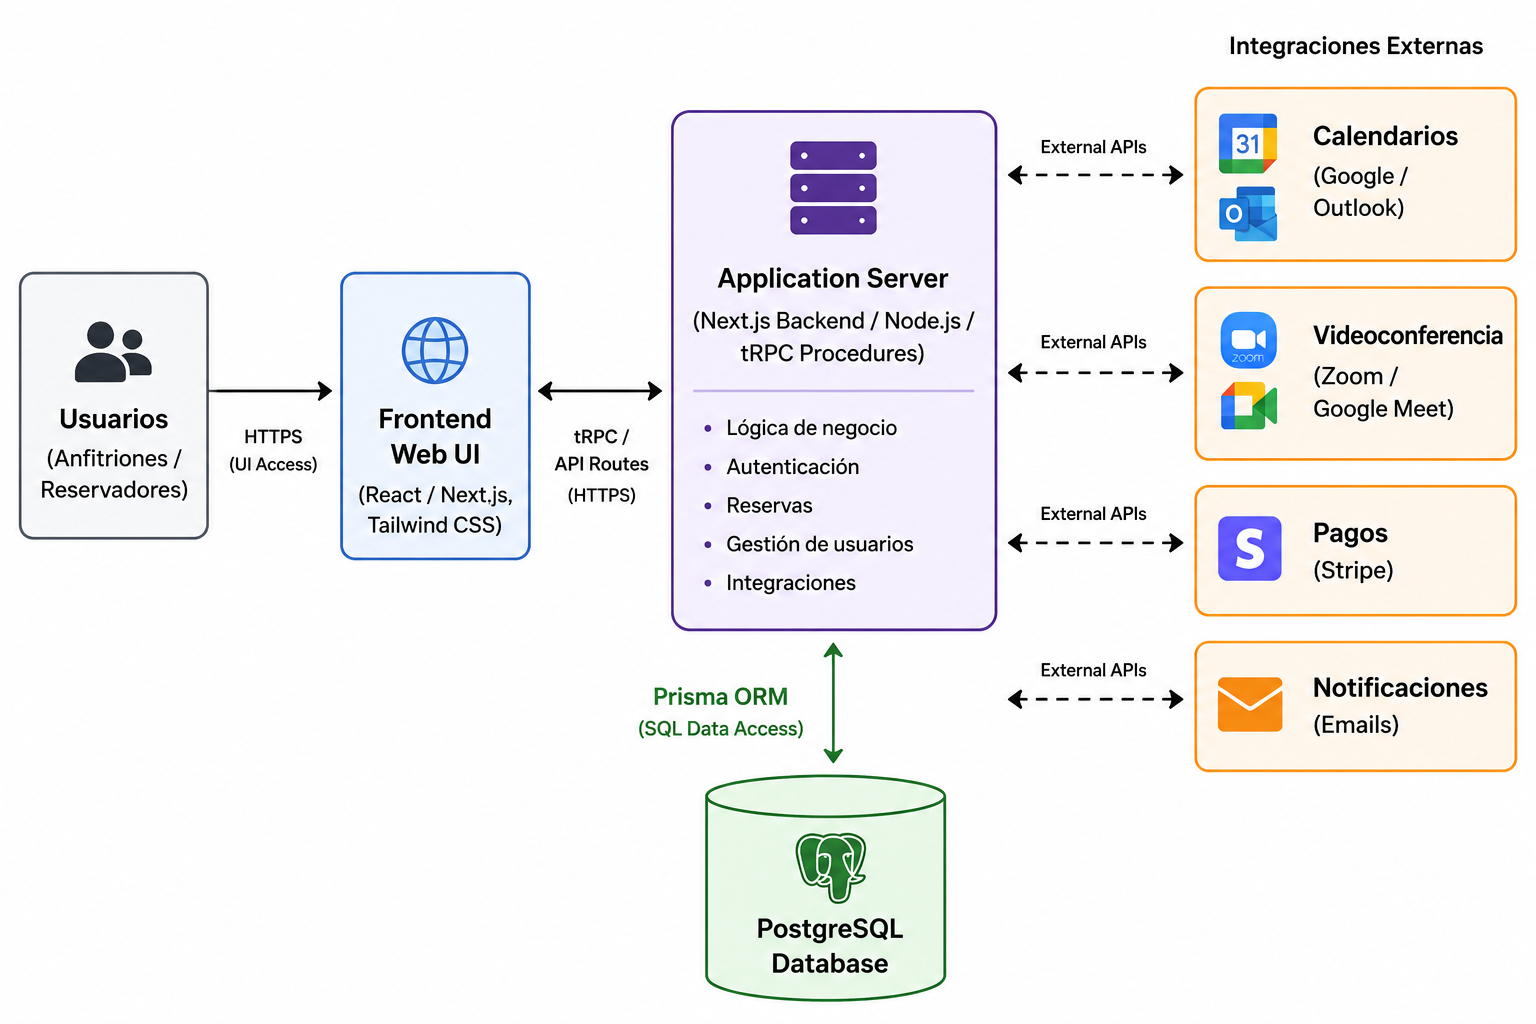
\includegraphics[width=0.9\textwidth]{diagrama.png}
    \caption{Diagrama de arquitectura de alto nivel de Cal.com, mostrando el flujo entre el Frontend, Backend, Base de Datos y servicios externos.}
    \label{fig:arquitectura}
\end{figure}

% ── 2.2 ISO/IEC 25010 ────────────────────────────────────────────────
\subsection{Análisis de calidad con ISO/IEC 25010}

La norma \textbf{ISO/IEC 25010} \parencite{iso25010} define el modelo de calidad del producto software
(\textit{SQuaRE} — Software Quality Requirements and Evaluation) \parencite{pressman2020}. Establece \textbf{8
características de calidad del producto} y \textbf{5 características de calidad en uso},
cada una con sus subcaracterísticas asociadas. A continuación se analiza detalladamente
cada característica en el contexto específico de cal.com.

% ── 2.2.1 ──
\subsubsection{Adecuación Funcional}

\textbf{Definición:} grado en que el software provee funciones que satisfacen las
necesidades declaradas e implícitas cuando se utiliza bajo condiciones especificadas.

En el caso de cal.com, la adecuación funcional es la característica de \textbf{mayor
prioridad}, dado que el valor central del sistema reside precisamente en la correcta
gestión del ciclo de agendamiento.

\begin{longtable}{>{\bfseries}p{3cm} p{4.5cm} p{4cm} p{3.5cm}}
\caption{Adecuación Funcional — cal.com} \label{tab:funcional} \\
\rowcolor{azulClaro}
\textcolor{white}{\textbf{Subcaracterística}} &
\textcolor{white}{\textbf{Descripción aplicada a cal.com}} &
\textcolor{white}{\textbf{Criterio de evaluación}} &
\textcolor{white}{\textbf{Observaciones}} \\
\endfirsthead
\multicolumn{4}{c}{\tablename\ \thetable{} -- continuación} \\
\rowcolor{azulClaro}
\textcolor{white}{\textbf{Subcaracterística}} &
\textcolor{white}{\textbf{Descripción aplicada a cal.com}} &
\textcolor{white}{\textbf{Criterio de evaluación}} &
\textcolor{white}{\textbf{Observaciones}} \\
\endhead
\rowpair
Completitud funcional &
cal.com cubre el ciclo completo de agendamiento: creación de tipos de eventos, gestión
de disponibilidad, integración con calendarios, envío de notificaciones y páginas de
reserva personalizadas. &
¿Cubre todos los flujos declarados en la documentación oficial? &
Alta: el conjunto de funcionalidades está bien documentado y cubierto. \\
\rowimpar
Corrección funcional &
Los cálculos de disponibilidad, zonas horarias y detección de conflictos deben producir
resultados exactos y consistentes. &
Pruebas de exactitud en detección de conflictos y zonas horarias. &
Crítico: errores aquí impactan directamente la experiencia del usuario. \\
\rowpair
Pertinencia funcional &
Las funciones expuestas (tipos de eventos, webhooks, integraciones) son relevantes para
el dominio de agendamiento empresarial y personal. &
Evaluación de si existen funciones que no aportan valor al usuario objetivo. &
El \textit{roadmap} público muestra alineación continua con necesidades reales. \\
\end{longtable}

% ── 2.2.2 ──
\subsubsection{Eficiencia de Desempeño}

\textbf{Definición:} desempeño relativo a la cantidad de recursos utilizados bajo
condiciones determinadas. En cal.com esta característica es \textbf{crítica} para la
página de reserva pública, cuyo tiempo de carga incide directamente en la tasa de
conversión.

\begin{longtable}{>{\bfseries}p{3cm} p{4.5cm} p{4cm} p{3.5cm}}
\caption{Eficiencia de Desempeño — cal.com} \label{tab:desempeno} \\
\rowcolor{azulClaro}
\textcolor{white}{\textbf{Subcaracterística}} &
\textcolor{white}{\textbf{Descripción aplicada a cal.com}} &
\textcolor{white}{\textbf{Criterio de evaluación}} &
\textcolor{white}{\textbf{Observaciones}} \\
\endfirsthead
\multicolumn{4}{c}{\tablename\ \thetable{} -- continuación} \\
\endhead
\rowpair
Comportamiento temporal &
Cal.com usa Next.js con SSR/SSG para optimizar tiempos de respuesta en la página de
reserva pública. &
Tiempo de carga $< 2\,\text{s}$ en conexión estándar; Core Web Vitals (LCP, FID, CLS). &
Se evalúa con Lighthouse y WebPageTest. \\
\rowimpar
Utilización de recursos &
El backend en Node.js y la base de datos PostgreSQL deben gestionar correctamente el
uso de CPU y memoria ante picos de carga. &
Monitoreo de consumo de CPU/RAM en producción bajo carga concurrente. &
Herramientas: Prometheus, Grafana o New Relic. \\
\rowpair
Capacidad &
La plataforma debe soportar múltiples usuarios simultáneos reservando \textit{slots} sin
degradación de servicio. &
Pruebas de carga con k6 o Locust para medir usuarios concurrentes. &
Aplicable especialmente en la versión \textit{self-hosted}. \\
\end{longtable}

% ── 2.2.3 ──
\subsubsection{Compatibilidad}

\textbf{Definición:} grado en que el sistema puede intercambiar información y/o realizar
sus funciones requeridas cuando comparte entorno con otros sistemas. Cal.com depende
estructuralmente de integraciones externas, lo que convierte esta característica en un
factor de riesgo relevante.

\begin{longtable}{>{\bfseries}p{3cm} p{4.5cm} p{4cm} p{3.5cm}}
\caption{Compatibilidad — cal.com} \label{tab:compat} \\
\rowcolor{azulClaro}
\textcolor{white}{\textbf{Subcaracterística}} &
\textcolor{white}{\textbf{Descripción aplicada a cal.com}} &
\textcolor{white}{\textbf{Criterio de evaluación}} &
\textcolor{white}{\textbf{Observaciones}} \\
\endfirsthead
\multicolumn{4}{c}{\tablename\ \thetable{} -- continuación} \\
\endhead
\rowpair
Coexistencia &
Cal.com puede ejecutarse junto a otros servicios en contenedores Docker sin
interferencias de puertos o recursos compartidos. &
Verificación de conflictos de puertos, variables de entorno o dependencias compartidas. &
Documentado en el \texttt{docker-compose} oficial. \\
\rowimpar
Interoperabilidad &
Integración con Google Calendar, Outlook, iCal, Zoom, Google Meet, Stripe y más de 100
integraciones vía API REST y webhooks. &
Pruebas de integración \textit{end-to-end} con cada proveedor externo. &
Se verifica en la sección de integraciones de la documentación oficial. \\
\end{longtable}

% ── 2.2.4 ──
\subsubsection{Usabilidad}

\textbf{Definición:} grado en que el sistema puede ser utilizado por usuarios específicos
para lograr metas específicas con efectividad, eficiencia y satisfacción. Esta
característica es especialmente relevante para los \textbf{usuarios reservadores}, quienes
interactúan con la plataforma sin necesariamente conocerla previamente.

\begin{longtable}{>{\bfseries}p{3cm} p{4.5cm} p{4cm} p{3.5cm}}
\caption{Usabilidad — cal.com} \label{tab:usabilidad} \\
\rowcolor{azulClaro}
\textcolor{white}{\textbf{Subcaracterística}} &
\textcolor{white}{\textbf{Descripción aplicada a cal.com}} &
\textcolor{white}{\textbf{Criterio de evaluación}} &
\textcolor{white}{\textbf{Observaciones}} \\
\endfirsthead
\multicolumn{4}{c}{\tablename\ \thetable{} -- continuación} \\
\endhead
\rowpair
Reconocibilidad apropiada &
Un usuario nuevo debe identificar rápidamente el propósito de la plataforma al llegar a
la página de reservas públicas. &
Test de comprensión de 5 segundos con usuarios nuevos. &
Evaluar con pruebas de usuario moderadas. \\
\rowimpar
Aprendibilidad &
El flujo de configuración inicial (cuenta, disponibilidad, primer tipo de evento) debe
completarse sin documentación adicional. &
Tiempo promedio en completar la configuración inicial. &
Objetivo: menos de 10 minutos para el primer evento publicado. \\
\rowpair
Operabilidad &
Los controles del \textit{dashboard} deben ser intuitivos: calendario de disponibilidad,
\textit{toggles} de integraciones y configuración de tipos de eventos. &
Tasa de errores de usuario en flujos principales (crear evento, ver reservas, conectar
calendario). &
Evaluable con \textit{session recording} (ej. Hotjar). \\
\rowimpar
Accesibilidad &
La interfaz web debe cumplir WCAG 2.1 nivel AA para usuarios con discapacidad. &
Auditoría con axe-core o Lighthouse Accessibility. &
Cal.com usa Tailwind y Radix UI, con soporte parcial de accesibilidad. \\
\rowpair
Protección contra errores &
El sistema debe evitar que el usuario reserve \textit{slots} fuera de disponibilidad o
cree conflictos en el calendario. &
Verificación de validaciones en formularios de reserva y configuración. &
Validaciones presentes en \textit{frontend} y \textit{backend}. \\
\end{longtable}

% ── 2.2.5 ──
\subsubsection{Fiabilidad}

\textbf{Definición:} grado en que el sistema realiza funciones específicas bajo
condiciones determinadas durante un período de tiempo. En un sistema de agendamiento,
la fiabilidad es \textbf{crítica}: un fallo en producción implica reservas perdidas y
daño a la reputación del anfitrión.

\begin{longtable}{>{\bfseries}p{3cm} p{4.5cm} p{4cm} p{3.5cm}}
\caption{Fiabilidad — cal.com} \label{tab:fiabilidad} \\
\rowcolor{azulClaro}
\textcolor{white}{\textbf{Subcaracterística}} &
\textcolor{white}{\textbf{Descripción aplicada a cal.com}} &
\textcolor{white}{\textbf{Criterio de evaluación}} &
\textcolor{white}{\textbf{Observaciones}} \\
\endfirsthead
\multicolumn{4}{c}{\tablename\ \thetable{} -- continuación} \\
\endhead
\rowpair
Madurez &
La plataforma debe operar sin fallos bajo uso normal y continuo. &
Tasa de fallos por período de tiempo (MTBF). &
Medible con monitoreo activo en producción. \\
\rowimpar
Disponibilidad &
El servicio debe estar disponible el mayor porcentaje de tiempo posible. &
Porcentaje de \textit{uptime} mensual. Objetivo: $\geq 99.5\,\%$. &
Herramientas: UptimeRobot, Pingdom o Statuspage. \\
\rowpair
Tolerancia a fallos &
Ante fallos de servicios externos (Google Calendar, Stripe), el sistema debe degradarse
graciosamente sin caídas completas. &
Comportamiento ante desconexión de APIs externas. &
Pruebas de \textit{chaos engineering} o \textit{mocking} de errores. \\
\rowimpar
Recuperabilidad &
Ante una caída, el sistema debe recuperarse y restaurar el servicio en el menor tiempo
posible. &
Tiempo de recuperación (MTTR). &
Monitoreo de \textit{deployments} y \textit{rollback} automático en CI/CD. \\
\end{longtable}

% ── 2.2.6 ──
\subsubsection{Seguridad}

\textbf{Definición:} grado en que el sistema protege la información y los datos de modo
que personas u otros sistemas tengan el acceso apropiado según su tipo y nivel de
autorización. Cal.com gestiona datos de calendario, contactos e información de pago, lo
que confiere \textbf{alta prioridad} a esta característica.

\begin{longtable}{>{\bfseries}p{3cm} p{4.5cm} p{4cm} p{3.5cm}}
\caption{Seguridad — cal.com} \label{tab:seguridad} \\
\rowcolor{azulClaro}
\textcolor{white}{\textbf{Subcaracterística}} &
\textcolor{white}{\textbf{Descripción aplicada a cal.com}} &
\textcolor{white}{\textbf{Criterio de evaluación}} &
\textcolor{white}{\textbf{Observaciones}} \\
\endfirsthead
\multicolumn{4}{c}{\tablename\ \thetable{} -- continuación} \\
\endhead
\rowpair
Confidencialidad &
Los datos de usuarios, calendarios y reservas deben estar cifrados en tránsito
(HTTPS/TLS) y en reposo. &
Verificación de certificados SSL y cifrado de campos sensibles en base de datos. &
En \textit{cloud} usa HTTPS; en \textit{self-hosted}, responsabilidad del operador. \\
\rowimpar
Integridad &
Los datos de reservas no deben ser modificados por terceros no autorizados. &
Pruebas de manipulación de datos en \textit{endpoints} de la API pública. &
Revisión de políticas de autorización en el código fuente (Next.js API routes). \\
\rowpair
No repudio &
Las acciones críticas (crear/cancelar reservas) deben quedar registradas con
identificación del actor. &
Existencia de \textit{logs} de auditoría en operaciones sensibles. &
Verificar la presencia de \textit{audit logs} en el repositorio. \\
\rowimpar
Autenticación &
El acceso al \textit{dashboard} requiere autenticación robusta. Cal.com soporta Google
OAuth, GitHub OAuth y credenciales propias. &
Implementación de OAuth2, manejo de \textit{tokens} y sesiones seguras. &
Implementado con NextAuth.js. \\
\rowpair
Autorización &
Los usuarios solo deben acceder y modificar sus propios eventos, disponibilidades y
reservas. &
Pruebas de acceso cruzado entre cuentas (IDOR — \textit{Insecure Direct Object
Reference}). &
Crítico en entornos multi-tenant. \\
\end{longtable}

% ── 2.2.7 ──
\subsubsection{Mantenibilidad}

\textbf{Definición:} grado de efectividad y eficiencia con la que el sistema puede ser
modificado para mejorarlo, corregirlo o adaptarlo. Cal.com es un proyecto de comunidad
activa con cientos de contribuidores, por lo que la mantenibilidad es un factor
\textbf{estratégico} para la sostenibilidad del proyecto.

\begin{longtable}{>{\bfseries}p{3cm} p{4.5cm} p{4cm} p{3.5cm}}
\caption{Mantenibilidad — cal.com} \label{tab:mantenibilidad} \\
\rowcolor{azulClaro}
\textcolor{white}{\textbf{Subcaracterística}} &
\textcolor{white}{\textbf{Descripción aplicada a cal.com}} &
\textcolor{white}{\textbf{Criterio de evaluación}} &
\textcolor{white}{\textbf{Observaciones}} \\
\endfirsthead
\multicolumn{4}{c}{\tablename\ \thetable{} -- continuación} \\
\endhead
\rowpair
Modularidad &
El repositorio está estructurado como \textit{monorepo} con paquetes separados
(\texttt{apps/web}, \texttt{packages/}). Cada módulo debe tener baja dependencia con
otros. &
Análisis de acoplamiento y cohesión con herramientas estáticas. &
Herramientas: Madge, ESLint, SonarQube. \\
\rowimpar
Reusabilidad &
Los componentes de UI (shadcn/ui y Tailwind) deben reutilizarse entre secciones de la
aplicación. &
Porcentaje de componentes reutilizados vs. duplicados. &
Análisis del directorio \texttt{packages/ui} del repositorio. \\
\rowpair
Analizabilidad &
Ante un \textit{bug} reportado, el desarrollador debe localizar el origen del error
eficientemente. &
Tiempo promedio en localizar un defecto reportado; existencia de \textit{logging}
estructurado. &
Herramienta: Sentry para \textit{error tracking}. \\
\rowimpar
Modificabilidad &
El código debe poder modificarse sin introducir defectos colaterales. &
Tasa de defectos introducidos por cambios (\textit{change failure rate}). &
Medible en CI/CD con métricas DORA. \\
\rowpair
Testeabilidad &
El sistema debe contar con pruebas unitarias, de integración y E2E. &
Cobertura de código (\textit{line/branch coverage}); existencia de pruebas E2E. &
Cal.com usa Playwright para E2E y Vitest para unitarias. \\
\end{longtable}

% ── 2.2.8 ──
\subsubsection{Portabilidad}

\textbf{Definición:} grado de efectividad y eficiencia con la que el sistema puede ser
transferido de un entorno de hardware, software u operativo a otro. Esta característica
es especialmente relevante dado que cal.com promueve activamente el auto-hospedaje como
propuesta de valor diferenciadora.

\begin{longtable}{>{\bfseries}p{3cm} p{4.5cm} p{4cm} p{3.5cm}}
\caption{Portabilidad — cal.com} \label{tab:portabilidad} \\
\rowcolor{azulClaro}
\textcolor{white}{\textbf{Subcaracterística}} &
\textcolor{white}{\textbf{Descripción aplicada a cal.com}} &
\textcolor{white}{\textbf{Criterio de evaluación}} &
\textcolor{white}{\textbf{Observaciones}} \\
\endfirsthead
\multicolumn{4}{c}{\tablename\ \thetable{} -- continuación} \\
\endhead
\rowpair
Adaptabilidad &
Cal.com puede desplegarse en distintos entornos: Vercel, AWS, VPS con Docker, Railway o
Render sin modificaciones al código fuente. &
Verificación de variables de entorno bien documentadas y ausencia de dependencias
\textit{hardcodeadas}. &
Revisión del repositorio y documentación de \textit{self-hosting}. \\
\rowimpar
Instalabilidad &
El proceso de instalación en un entorno nuevo (\textit{self-hosted}) debe ser
documentado y ejecutable sin conocimientos expertos. &
Número de pasos y tiempo estimado de \textit{setup}. &
Cal.com provee \texttt{docker-compose} y guía de \textit{self-hosting}. \\
\rowpair
Reemplazabilidad &
La plataforma debe poder sustituirse por otra solución de agendamiento con mínima
pérdida de datos (exportación de reservas, contactos y configuraciones). &
Existencia de funciones de exportación de datos (CSV, API). &
Evaluable desde el \textit{dashboard} de cal.com. \\
\end{longtable}

\subsubsection*{Priorización de características}

Con base en el análisis anterior, la siguiente tabla resume la prioridad asignada a cada
característica para el contexto específico de cal.com:

\begin{center}
\begin{tabular}{clcc}
\toprule
\textbf{\#} & \textbf{Característica ISO/IEC 25010} & \textbf{Prioridad} & \textbf{Justificación} \\
\midrule
1 & Adecuación Funcional   & \textbf{Alta}  & Núcleo del valor del producto \\
2 & Fiabilidad             & \textbf{Alta}  & Fallos generan pérdida de reservas \\
3 & Seguridad              & \textbf{Alta}  & Gestión de datos sensibles \\
4 & Eficiencia de Desempeño & \textbf{Alta} & Impacta tasa de conversión \\
5 & Usabilidad             & \textbf{Media} & Clave para usuarios sin experiencia \\
6 & Mantenibilidad         & \textbf{Media} & Proyecto de comunidad activa \\
7 & Compatibilidad         & \textbf{Media} & Depende de integraciones externas \\
8 & Portabilidad           & \textbf{Baja}  & Valorada pero no crítica en uso diario \\
\bottomrule
\end{tabular}
\end{center}

\subsubsection*{Características de Calidad en Uso}
De acuerdo con la norma ISO/IEC 25010 \parencite{iso25010}, además de la calidad interna del producto, se deben considerar las 5 características de Calidad en Uso: Efectividad, Eficiencia, Satisfacción, Mitigación de Riesgos y Cobertura de Contexto. Para el ecosistema de cal.com, las dos más relevantes a discutir son:

\begin{itemize}
    \item \textbf{Satisfacción:} Es crítica para los \textit{usuarios reservadores}. Si la experiencia de agendar (UI/UX) no genera confianza, fluidez y comodidad, el usuario abandona el proceso, afectando directamente el valor de la herramienta.
    \item \textbf{Mitigación de Riesgos (Económicos y Reputacionales):} Un fallo en el sistema de reservas, zonas horarias o en las integraciones de pago (ej. Stripe) tiene un impacto financiero directo e inmediato para el anfitrión (pérdida de ingresos o clientes).
\end{itemize}

% ── 2.3 KPIs ISO/IEC 25023 ───────────────────────────────────────────
\subsection{KPIs medibles según ISO/IEC 25023}

La norma \textbf{ISO/IEC 25023} \parencite{iso25023} define las medidas de calidad del producto software que
complementan el modelo de la ISO/IEC 25010. A continuación se presentan los KPIs más
representativos para cal.com, organizados por característica, con fórmula matemática,
valor objetivo y herramienta de medición recomendada.

% ─── Funcional
\subsubsection*{Adecuación Funcional}

\begin{enumerate}[leftmargin=*, label=\textbf{KPI \arabic*.}]

    \item \textbf{Completitud de casos de uso implementados}
    \[
        \text{Completitud} = \frac{\text{Casos implementados}}{\text{Casos requeridos}} \times 100 \geq 95\,\%
    \]
    \textit{Herramienta:} revisión del \textit{backlog} en GitHub Issues.

    \item \textbf{Tasa de defectos funcionales}
    \[
        \text{TDF} = \frac{\text{Defectos funcionales}}{\text{Total de funciones}} \times 100 < 2\,\%
    \]
    \textit{Herramienta:} Sentry / GitHub Issues.

    \item \textbf{Tasa de reservas completadas}
    \[
        \text{TRC} = \frac{\text{Reservas completadas}}{\text{Intentos de reserva}} \times 100 \geq 98\,\%
    \]
    \textit{Herramienta:} \textit{analytics} y \textit{logs} de base de datos.

\end{enumerate}

% ─── Desempeño
\subsubsection*{Eficiencia de Desempeño}

\begin{enumerate}[leftmargin=*, label=\textbf{KPI \arabic*.}, start=4]

    \item \textbf{Largest Contentful Paint (LCP)}
    \[
        \text{LCP} < 2.5\,\text{s}
    \]
    \textit{Herramienta:} Lighthouse / Chrome UX Report (CrUX).

    \item \textbf{First Input Delay (FID)}
    \[
        \text{FID} < 100\,\text{ms}
    \]
    \textit{Herramienta:} Lighthouse / CrUX.

    \item \textbf{Tiempo de respuesta de API (percentil 95)}
    \[
        T_{\text{respuesta}}^{p95} < 500\,\text{ms}
    \]
    \textit{Herramienta:} k6, Postman Monitor.

    \item \textbf{Usuarios concurrentes soportados}
    \[
        U_{\text{concurrentes}} \geq 500 \text{ sin degradación} > 20\,\%
    \]
    \textit{Herramienta:} k6 / Locust.

\end{enumerate}

% ─── Compatibilidad
\subsubsection*{Compatibilidad}

\begin{enumerate}[leftmargin=*, label=\textbf{KPI \arabic*.}, start=8]

    \item \textbf{Tasa de éxito de integraciones}
    \[
        \text{TEI} = \frac{\text{Integraciones funcionales}}{\text{Integraciones documentadas}} \times 100 \geq 95\,\%
    \]
    \textit{Herramienta:} pruebas de integración E2E.

    \item \textbf{Éxito de sincronización de calendario}
    \[
        \text{ESC} = \frac{\text{Eventos sincronizados correctamente}}{\text{Total de eventos}} \times 100 \geq 99\,\%
    \]
    \textit{Herramienta:} \textit{logs} de webhooks / Playwright.

\end{enumerate}

% ─── Usabilidad
\subsubsection*{Usabilidad}

\begin{enumerate}[leftmargin=*, label=\textbf{KPI \arabic*.}, start=10]

    \item \textbf{Tasa de finalización de tarea (onboarding)}
    \[
        \text{TFT} = \frac{\text{Usuarios que completan el setup inicial}}{\text{Total que inician}} \times 100 \geq 80\,\%
    \]
    \textit{Herramienta:} Hotjar / Mixpanel.

    \item \textbf{Tiempo promedio de configuración inicial}
    \[
        T_{\text{config}} < 10\,\text{min}
    \]
    \textit{Herramienta:} Mixpanel / PostHog.

    \item \textbf{Puntuación SUS (System Usability Scale)}
    \[
        \text{SUS} \geq 75 \quad \text{(sobre 100)}
    \]
    \textit{Herramienta:} encuesta SUS post-sesión de prueba.

    \item \textbf{Violaciones críticas de accesibilidad WCAG 2.1 AA}
    \[
        V_{\text{críticas}} = 0
    \]
    \textit{Herramienta:} axe-core / Lighthouse Accessibility.

\end{enumerate}

% ─── Fiabilidad
\subsubsection*{Fiabilidad}

\begin{enumerate}[leftmargin=*, label=\textbf{KPI \arabic*.}, start=14]

    \item \textbf{Disponibilidad del servicio (Uptime)}
    \[
        D = \frac{T_o}{T_o + T_d} \times 100 \geq 99.5\,\%
    \]
    donde $T_o$ = tiempo operativo y $T_d$ = tiempo de inactividad. \textit{Herramienta:} UptimeRobot / Pingdom.

    \item \textbf{MTBF (Mean Time Between Failures)}
    \[
        \text{MTBF} = \frac{\sum T_{\text{operativo}}}{\text{Número de fallos}} \geq 720\,\text{h}
    \]
    \textit{Herramienta:} Grafana / PagerDuty.

    \item \textbf{MTTR (Mean Time To Recovery)}
    \[
        \text{MTTR} = \frac{\sum T_{\text{recuperación}}}{\text{Número de incidentes}} < 30\,\text{min}
    \]
    \textit{Herramienta:} PagerDuty / Statuspage.

    \item \textbf{Tasa de errores del sistema (5xx)}
    \[
        \text{TE} = \frac{\text{Errores 5xx}}{\text{Total de \textit{requests}}} \times 100 < 0.1\,\%
    \]
    \textit{Herramienta:} Sentry / Datadog.

\end{enumerate}

% ─── Seguridad
\subsubsection*{Seguridad}

\begin{enumerate}[leftmargin=*, label=\textbf{KPI \arabic*.}, start=18]

    \item \textbf{Cobertura HTTPS/TLS}
    \[
        C_{\text{TLS}} = \frac{\text{Endpoints con HTTPS}}{\text{Total de endpoints}} \times 100 = 100\,\%
    \]
    \textit{Herramienta:} SSL Labs / OWASP ZAP.

    \item \textbf{Vulnerabilidades críticas abiertas}
    \[
        V_{\text{críticos}} = 0 \quad \text{(CVEs críticos sin parchear)}
    \]
    \textit{Herramienta:} Snyk / Dependabot.

    \item \textbf{Tiempo de respuesta a vulnerabilidades críticas}
    \[
        T_{\text{respuesta}} < 7\,\text{días desde reporte}
    \]
    \textit{Herramienta:} GitHub Security Advisories.

\end{enumerate}

% ─── Mantenibilidad
\subsubsection*{Mantenibilidad}

\begin{enumerate}[leftmargin=*, label=\textbf{KPI \arabic*.}, start=21]

    \item \textbf{Cobertura de pruebas (código)}
    \[
        C_{\text{pruebas}} = \frac{\text{Líneas cubiertas por tests}}{\text{Total de líneas}} \times 100 \geq 80\,\%
    \]
    \textit{Herramienta:} Vitest + Istanbul.

    \item \textbf{Change Failure Rate (CFR)}
    \[
        \text{CFR} = \frac{\text{Deployments con fallo}}{\text{Total de deployments}} \times 100 < 15\,\%
    \]
    \textit{Herramienta:} GitHub Actions / Vercel.

    \item \textbf{Lead Time for Changes}
    \[
        LT < 1\,\text{día (desde commit hasta producción)}
    \]
    \textit{Herramienta:} métricas DORA / LinearB.

    \item \textbf{Deuda técnica (Technical Debt Ratio)}
    \[
        \text{TDR} = \frac{\text{Tiempo estimado de remediación}}{\text{Tiempo de desarrollo}} \times 100 < 5\,\%
    \]
    \textit{Herramienta:} SonarQube.

\end{enumerate}

% ─── Portabilidad
\subsubsection*{Portabilidad}

\begin{enumerate}[leftmargin=*, label=\textbf{KPI \arabic*.}, start=25]

    \item \textbf{Tiempo de instalación self-hosted}
    \[
        T_{\text{install}} < 30\,\text{min (desde \texttt{git clone} hasta sistema funcional)}
    \]
    \textit{Herramienta:} prueba manual documentada.

    \item \textbf{Compatibilidad de entornos de despliegue}
    \[
        E_{\text{probados}} \geq 3 \quad \text{(entornos verificados y documentados)}
    \]
    \textit{Herramienta:} \textit{matrix testing} en CI/CD.

    \item \textbf{Cobertura de exportación de datos}
    \[
        C_{\text{export}} = 100\,\% \text{ de entidades críticas (reservas, contactos, configuraciones)}
    \]
    \textit{Herramienta:} prueba manual de exportación.

\end{enumerate}

\subsubsection*{Notas de implementación para la medición de KPIs}

Para garantizar la trazabilidad y reproducibilidad de las métricas definidas, el equipo
recomienda las siguientes prácticas:

\begin{itemize}
    \item Establecer un \textit{baseline} inicial antes de aplicar mejoras, registrando el valor de cada KPI en el estado actual del sistema.
    \item Automatizar la recolección de métricas en el \textit{pipeline} de CI/CD (GitHub Actions) ejecutando Lighthouse, k6 y axe-core en cada \textit{release}.
    \item Configurar \textit{dashboards} de monitoreo en producción (Grafana + Prometheus o Datadog) para el seguimiento continuo de disponibilidad, errores y desempeño.
    \item Ejecutar evaluaciones de usabilidad con al menos 5 usuarios reales para las métricas de satisfacción y tasa de finalización de tareas.
    \item Revisar vulnerabilidades de seguridad con Snyk o Dependabot de forma semanal y registrar el tiempo de respuesta a cada hallazgo.
    \item Documentar cada medición con fecha, versión del sistema evaluado y condiciones de medición para facilitar comparaciones históricas.
\end{itemize}

% ── 2.4 Plan SQA ────────────────────────────────────────────────────
\subsection{Plan SQA preliminar según IEEE 730}

Para asegurar que las modificaciones e implementaciones sobre la plataforma cal.com mantengan un nivel óptimo, se define el siguiente Plan de Aseguramiento de Calidad de Software basado en el estándar \parencite{ieee730}.

\subsubsection*{Purpose (Alcance del plan)}
El propósito de este plan es definir los procesos, métricas y responsabilidades de SQA aplicables a la adaptación, despliegue y mantenimiento de cal.com. El alcance cubre desde la validación del código fuente mediante análisis estático hasta las pruebas de integración en entornos de auto-hospedaje (\textit{self-hosted}).

\subsubsection*{Management (Roles)}
El equipo de trabajo se distribuye en los siguientes roles de calidad:
\begin{itemize}
    \item \textbf{Líder SQA:} Responsable de auditar el cumplimiento del estándar y autorizar los pases a producción.
    \item \textbf{Ingeniero de Pruebas (QA):} Encargado de diseñar y ejecutar pruebas E2E en Playwright y reportar defectos.
    \item \textbf{Desarrollador / DevOps:} Responsable de ejecutar pruebas unitarias con Vitest y mantener el pipeline de CI/CD.
\end{itemize}

\subsubsection*{Standards, practices, metrics}
Se adoptan las métricas definidas en la sección 2.3 de este documento (basadas en ISO/IEC 25023). Adicionalmente, se imponen las siguientes prácticas auditables:
\begin{itemize}
    \item Uso estricto de \textbf{ESLint} y \textbf{Prettier} para estandarizar el formato del código TypeScript.
    \item Análisis de código estático obligatorio con \textbf{SonarQube} en cada \textit{Pull Request}.
    \item Prohibición técnica de integrar código que reduzca la cobertura de pruebas actual del repositorio.
\end{itemize}

\subsubsection*{Test (Estrategia de pruebas)}
La estrategia se divide en tres niveles integrados en GitHub Actions:
\begin{itemize}
    \item \textbf{Pruebas Unitarias:} Ejecutadas localmente y en el pipeline usando Vitest para la lógica de negocio y cálculos de zonas horarias.
    \item \textbf{Pruebas E2E:} Ejecutadas con Playwright para simular el flujo completo de reserva de un usuario real en un navegador \textit{headless}.
    \item \textbf{Pruebas de Carga:} Evaluaciones periódicas con k6 para validar la subcaracterística de Capacidad de desempeño.
\end{itemize}

\subsubsection*{Problem reporting}
Los defectos encontrados se gestionarán mediante GitHub Issues y Sentry, clasificados por severidad con los siguientes SLA (Acuerdos de Nivel de Servicio):
\begin{itemize}
    \item \textbf{Crítico (Caída del sistema o brecha de seguridad):} Tiempo de respuesta inmediato; resolución en menos de 24 horas.
    \item \textbf{Mayor (Fallo funcional sin alternativa u \textit{workaround}):} Resolución en el sprint actual (máximo 7 días).
    \item \textbf{Menor (Errores de UI/UX o fallos visuales):} Envío al backlog para priorización mensual.
\end{itemize}

% ── 2.5 Modelo de madurez ───────────────────────────────────────────
\subsection{Recomendación de modelo de madurez}
Para un equipo pequeño (4 integrantes) encargado de adaptar e implementar cal.com, es fundamental seleccionar un modelo de madurez de procesos que sea realista, aplicable y económicamente viable. Tras evaluar CMMI, ISO/IEC 33000 y MoProSoft, se concluye lo siguiente:

\textbf{CMMI (Capability Maturity Model Integration)} es el estándar de facto a nivel internacional para grandes corporativos, pero su implementación resulta pesada, burocrática y costosa para equipos ágiles pequeños. Por otro lado, \textbf{ISO/IEC 33000} ofrece un marco robusto de evaluación, pero su alto nivel de abstracción dificulta una adopción rápida sin consultoría externa.

Por lo tanto, se recomienda adoptar \textbf{MoProSoft (NMX-I-059-NYCE)} como el modelo de madurez ideal para el contexto de este proyecto. MoProSoft fue diseñado específicamente para la industria de software en México y está optimizado para Pequeñas y Medianas Empresas (PyMEs) \parencite{oktaba2008}.

La justificación técnica para elegir MoProSoft se fundamenta en tres factores:
\begin{itemize}
\item \textbf{Tamaño del equipo:} La estructura organizacional de MoProSoft (Alta Dirección, Gerencia y Operación) se puede mapear ágilmente a un equipo de 4 personas utilizando el concepto de "roles" en lugar de departamentos rígidos.
\item \textbf{Orientación práctica:} Proporciona procesos claramente definidos (como Gestión de Proyectos y Desarrollo/Mantenimiento de Software) que encajan de forma natural con el trabajo de personalización y despliegue del monorepo de cal.com.
\item \textbf{Mercado objetivo:} Si el equipo proyecta ofrecer cal.com como servicio comercial gestionado en el mercado mexicano o latinoamericano, la certificación MoProSoft avala la calidad del proceso localmente y sirve como el escalón preparatorio ideal hacia futuras certificaciones ISO.
\end{itemize}

% ── 2.6 Matriz de riesgos ───────────────────────────────────────────
\subsection{Matriz de riesgos de calidad}

Con base en el análisis de calidad ISO/IEC 25010 realizado, se identificaron los siguientes riesgos principales asociados a los atributos de calidad de cal.com, apoyándonos en las metodologías de gestión de riesgos de calidad \parencite{galin2018}:

\begin{longtable}{>{\bfseries\centering}p{0.5cm} p{3.8cm} p{2.5cm} p{1cm} p{1cm} p{4cm}}
\caption{Matriz de Riesgos de Calidad — cal.com} \label{tab:riesgos} \\
\rowcolor{azulUPA}
\textcolor{white}{\textbf{\#}} &
\textcolor{white}{\textbf{Descripción}} &
\textcolor{white}{\textbf{Atributo ISO}} &
\textcolor{white}{\textbf{Prob.}} &
\textcolor{white}{\textbf{Imp.}} &
\textcolor{white}{\textbf{Mitigación}} \\
\endfirsthead
\multicolumn{6}{c}{\tablename\ \thetable{} -- continuación} \\
\endhead
\rowpair
1 & Error en cálculo de zonas horarias genera reservas en horario incorrecto. &
Adecuación Funcional & A & A &
Pruebas unitarias exhaustivas de conversión de zonas horarias; \textit{fuzzing} con fechas límite y cambios de horario de verano. \\
\rowimpar
2 & Fallo de servicio externo (Google Calendar) causa caída total del agendamiento. &
Fiabilidad & M & A &
Implementar \textit{circuit breaker} y degradación graceful; \textit{queue} de sincronización asíncrona. \\
\rowpair
3 & Vulnerabilidad IDOR permite acceso a reservas de otro usuario. &
Seguridad & M & A &
Auditoría de endpoints de API; pruebas de autorización entre cuentas; revisión con OWASP ZAP. \\
\rowimpar
4 & Tiempo de carga $> 3\,\text{s}$ en página de reserva pública reduce tasa de conversión. &
Eficiencia de Desempeño & M & M &
Optimización de imágenes, \textit{lazy loading}, análisis de \textit{bundle size} con Lighthouse. \\
\rowpair
5 & Alta deuda técnica en módulos legacy dificulta incorporación de contribuidores. &
Mantenibilidad & M & M &
Análisis periódico con SonarQube; definir umbrales de deuda técnica en \textit{pull request} gates. \\
\rowimpar
6 & Proceso de \textit{self-hosting} complejo genera instalaciones incorrectas y soporte elevado. &
Portabilidad & B & M &
Mejorar documentación de instalación; publicar \textit{scripts} de validación post-instalación. \\
\end{longtable}

\noindent\textbf{Leyenda:} A = Alto, M = Medio, B = Bajo.

% ==========================================
% 5. CONCLUSIÓN INTEGRAL
% ==========================================
\section{Conclusión integral}

La aplicación de los estándares \textbf{ISO/IEC 25010} e \textbf{ISO/IEC 25023} al
sistema cal.com permitió al equipo trascender la evaluación subjetiva del software y
anclar el análisis en criterios objetivos, medibles y comparables. Entre los hallazgos
más relevantes se destacan los siguientes:

\begin{itemize}
    \item \textbf{Adecuación funcional:} cal.com cubre de forma completa el dominio de agendamiento. El mayor riesgo reside en la corrección de los cálculos de zonas horarias y la detección de conflictos, que son la base del valor diferencial de la plataforma.

    \item \textbf{Eficiencia de desempeño:} la arquitectura basada en Next.js con SSR/SSG favorece buenos tiempos de carga. Se recomienda monitoreo continuo de Core Web Vitals y pruebas de carga periódicas para entornos \textit{self-hosted}.

    \item \textbf{Compatibilidad:} el amplio ecosistema de integraciones es una fortaleza estratégica. Sin embargo, requiere pruebas E2E automatizadas por cada proveedor para garantizar disponibilidad continua.

    \item \textbf{Usabilidad:} la interfaz es moderna y relativamente intuitiva. Se recomienda aplicar el SUS (System Usability Scale) con usuarios reales y realizar una auditoría formal de accesibilidad WCAG 2.1.

    \item \textbf{Fiabilidad:} la versión cloud alcanza estándares aceptables de uptime. En \textit{self-hosted}, la fiabilidad depende de la infraestructura del operador y requiere documentación adicional.

    \item \textbf{Seguridad:} la implementación de OAuth2 vía NextAuth.js es adecuada. Se recomienda análisis estático con Snyk y pruebas OWASP ZAP periódicas, especialmente en endpoints multi-tenant.

    \item \textbf{Mantenibilidad:} la estructura de \textit{monorepo} y el uso de Playwright/Vitest son fortalezas. Se recomienda aumentar la cobertura de pruebas hasta el 80\% y monitorear métricas DORA de forma continua.

    \item \textbf{Portabilidad:} la disponibilidad de \texttt{docker-compose} y la guía de \textit{self-hosting} favorecen la portabilidad. Se recomienda validar y documentar el despliegue en al menos tres entornos distintos.
\end{itemize}

En total se definieron \textbf{27 KPIs medibles} alineados con ISO/IEC 25023,
distribuidos en las 8 características de calidad, con fórmulas, valores objetivo y
herramientas específicas para su medición en el contexto de cal.com. Este conjunto de
métricas constituye la base para el Plan SQA y la posterior evaluación de madurez del
proceso.

% ==========================================
% 6. APORTES INDIVIDUALES
% ==========================================
\section{Aportes individuales}

\textbf{Christopher Rubén Rosales Gómez (UP240507):} Coordinó el entorno de trabajo colaborativo en Git/GitHub, diseñó la arquitectura del documento base en LaTeX, implementó el motor BibTeX para el cumplimiento estricto del formato APA 7 y colaboró en la definición del contexto e introducción del proyecto. \\[0.3cm]

\textbf{Jesús Ernesto Navarro Guel (UP240193):} Investigó y redactó el Plan de Aseguramiento de Calidad (SQA) preliminar adaptando las directrices del estándar IEEE 730 al contexto del proyecto, y estructuró los niveles de la estrategia de pruebas (Sección 2.4). \\[0.3cm]

\textbf{Mía Lizeska Babún Pérez (UP260733):} Realizó el análisis comparativo de modelos de madurez (CMMI, ISO 33000 y MoProSoft), justificando técnica y operativamente la adopción de MoProSoft, y colaboró en las estrategias de mitigación (Sección 2.5). \\[0.3cm]

\textbf{Diego Sánchez González (UP240430):} Documentó el stack tecnológico del proyecto, evaluó la plataforma bajo las 8 características del estándar ISO/IEC 25010, estructuró las fórmulas de los KPIs basados en ISO/IEC 25023 y redactó la conclusión integral.
% ==========================================
% 7. REFERENCIAS
% ==========================================
\newpage
\section{Referencias}
\printbibliography

\end{document}